% sage_latex_guidelines.tex V1.10, 24 June 2016

\documentclass[Crown, sagev, times, doublespace]{sagej}

\usepackage{moreverb,url,amsmath,amssymb,graphicx,multirow,textcomp,color,epsfig,dcolumn,float,setspace,booktabs,float,subfig,rotating,adjustbox,chngcntr}
\usepackage[colorlinks,bookmarksopen,bookmarksnumbered,citecolor=red,urlcolor=red]{hyperref}

\counterwithin{subfigure}{figure}
\graphicspath{{figures/}}

\newcommand\BibTeX{{\rmfamily B\kern-.05em \textsc{i\kern-.025em b}\kern-.08em,
T\kern-.1667em\lower.7ex\hbox{E}\kern-.125emX}}

\def\volumeyear{2016}

\setcounter{secnumdepth}{3}
\begin{document}

\runninghead{Ming Yang et al.}

\title{Bayesian quantile regression joint models: inference and dynamic predictions}

\author{Ming Yang\affilnum{1}, Sheng Luo\affilnum{2} and Stacia DeSantis\affilnum{1}}

\affiliation{\affilnum{1}Department of Biostatistics, The University of Texas Health Science Center at Houston, 1200 Pressler St, Houston, TX 77030, USA
\affilnum{2} Department of Biostatistics and Bioinformatics, Duke University Medical Center, 2400 Pratt St, 7040 North Pavilion, Durham, NC 27705, USA}

\corrauth{Sheng Luo, Department of Biostatistics and Bioinformatics
Duke University Medical Center,
2400 Pratt St, 7040 North Pavilion, Durham, NC 27705, USA.}

\email{sheng.luo@duke.edu}

\begin{abstract}
In the traditional joint models (JM) of a longitudinal and time-to-event outcome, a linear mixed model (LMM) assuming normal random errors is used to model the longitudinal process. However, in many circumstances, the normality assumption is violated and the LMM is not an appropriate sub-model in the JM. In addition, as the LMM models the conditional mean of the longitudinal outcome, it is not appropriate if clinical interest lies in making inference or prediction on median, lower, or upper ends of the longitudinal process. To this end, quantile regression (QR) provides a flexible, distribution-free way to study covariate effects at different quantiles of the longitudinal outcome and it is robust not only to deviation from normality, but also to outlying observations. In this article, we present and advocate the linear quantile mixed model (LQMM) for the longitudinal process in the JM framework. Our development is motivated by a large prospective study of Huntington's Disease (HD) where primary clinical interest is in utilizing longitudinal motor scores and other early covariates to predict the risk of developing HD. We develop a Bayesian method based on the location-scale representation of the asymmetric Laplace distribution (ALD), assess its performance through an extensive simulation study, and demonstrate how this LQMM-based JM approach can be used for making subject-specific dynamic predictions of survival probability.
\end{abstract}

\keywords{Asymmetric Laplace distribution, Bayesian inference, Huntington's disease, Linear quantile mixed model, MCMC}

\maketitle

\section{Introduction}
Joint models (JM) of longitudinal and time-to-event data have been well developed in the literature as they are highly applicable in the settings of longitudinal data analysis with event-related terminal events (e.g., dropout or death which is related to the longitudinal process), or of survival analysis with time-dependent covariates measured with error.\citep{self1992modeling, tsiatis1995modeling} JM have been extensively studied in recent years and an excellent review is provided by Tsiatis and Davidian.\cite{tsiatis2004joint}

Within the traditional JM framework, a linear mixed model (LMM) is used to model the longitudinal continuous outcome. To account for within-subject correlation, measurements from the same individual share random effects, and random errors are assumed to be normally distributed.\citep{laird1982random} However, if normality assumption of the random errors is violated (even after applying various outcome transformations), an LMM is not appropriate. Further, an LMM  models covariate effects on the conditional mean of the longitudinal outcome. However, in many clinical studies it is of interest to make inference or prediction on median, lower or higher quantiles of the longitudinal outcome. For example, in a study of the impact of various health factors on low birth weight, which is closely associated with infant mortality and development of chronic diseases, researchers fit a quantile regression (QR) model and find several significantly different covariate effects on lower birth weight compared with that on the mean birth weight.\citep{koenker2001quantile} Thus, QR may serve as an alternative to conditional mean regression when the aforementioned limitations are present, or when the subject matter dictates.

In contrast to mean regression such as LMMs, original QR models offer a flexible framework that relaxes the distributional assumption, and provides a way to study covariate effects on various quantiles of the outcome.\citep{koenker2005quantile} QR has attracted much attention since the seminal work of Koenker and Bassett Jr,\cite{koenker1978regression} and extensions for longitudinal data have been explored by many authors.\citep{koenker2004quantile, geraci2007quantile, geraci2013linear, kozumi2011gibbs} Recently, Farcomeni and Viviani \cite{farcomeni2015longitudinal} first incorporated a linear quantile mixed model (LQMM) into a JM for longitudinal and survival processes, for which they utilized a Monte Carlo Expectation Maximization (MCEM) algorithm for parameter estimation.

Our work is motivated by the Neurobiological Predictors of Huntington's Disease (HD) study (PREDICT-HD; ClinicalTrials.gov number NCT00051324), a prospective observational study (n=1078) designed to detect early neurobiological predictors of HD. A total of 40 longitudinal biomarkers were measured during the study follow-up of 12 years, where the outcome of interest was time to motor diagnosis of HD (referred to as HD onset). As the primary focus of this study was to measure the association between longitudinal biomarkers and risk of HD onset, the clinical question lends itself to a joint modeling approach. The top panel of Figure~\ref{fig:data_neurotot} displays the scatter plot and kernel density (on the right side) of total motor score (TMS), a commonly used rating criteria of body motion abilities based on the Unified Huntington Disease Rating Scale (UHDRS). The top panel suggests that TMS increases (deteriorates) as time progresses. The bottom panel of Figure~\ref{fig:data_neurotot} displays the mean TMS values over time for individuals with follow-up time less than 48 months (solid line), 48$-$72 months (dotted line), and more than 72 months (slashed line). It indicates that individuals with shorter follow-up tend to have higher TMS values (worse mobility). Because individuals with higher TMS are at greater risk of developing HD, it is of particular interest to explore the disease progression in a higher TMS subpopulation as opposed to modeling the conditional mean of TMS.

\begin{figure}[ht]
\centering
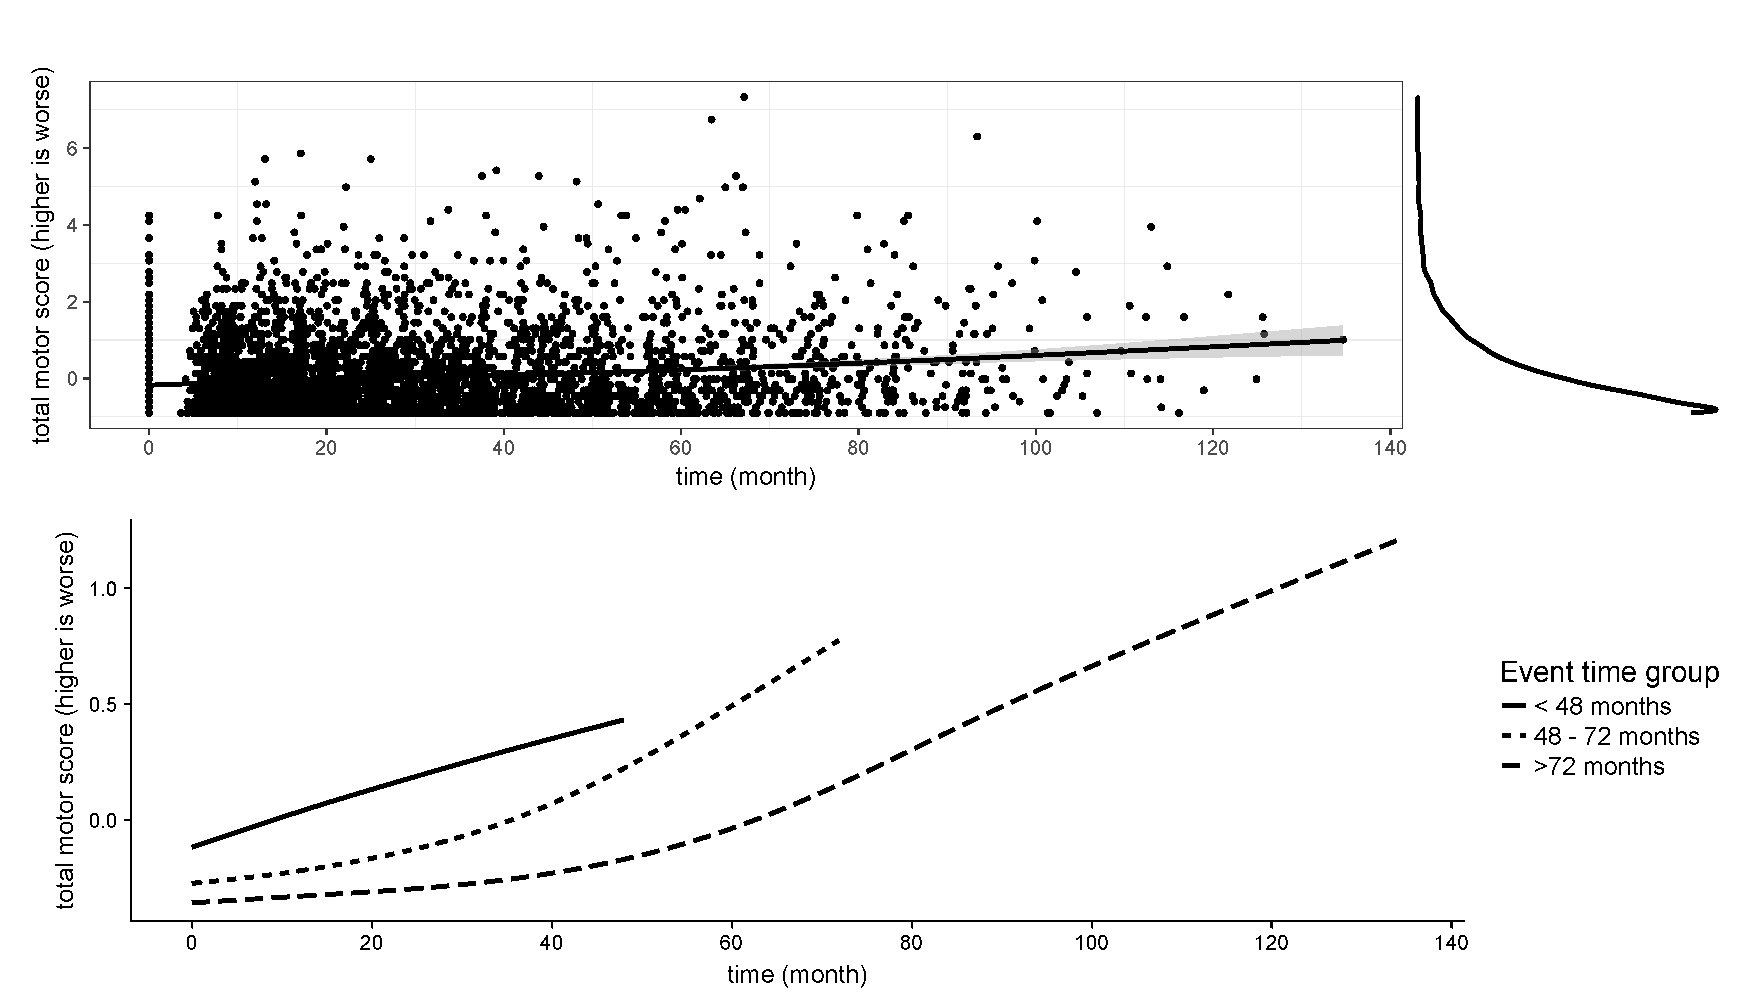
\includegraphics[width=1\textwidth]{TMS_bw.eps}
\caption{Top panel: Scatter plot (with loess curve) and kernel density plot (right side) for {total motor score} from the study population (time unit: month; lower total motor score is better); bottom panel: Mean total motor score values over time by event time group.}
\label{fig:data_neurotot}
\end{figure}

Moreover, we are specifically interested in estimating the risk of developing HD for those individuals who are still free of the disease. To this end, the JM framework offers a novel way of making such personalized dynamic predictions of future event-free probability.\citep{rizopoulos2011dynamic,taylor2013real} A key feature of these dynamic predictions frameworks is that the predictive measures can be dynamically updated as additional longitudinal measurements from the target individual become available, providing instantaneous risk assessment. To make dynamic predictions in the current context, we first build the quantile regression joint model (QRJM) consisting of a LQMM for the longitudinal process and a Cox proportional hazard model (PHM) for the time to HD onset process and then draw Bayesian inference, based on a large study population. Next, conditioning on an individual's longitudinal biomarker trajectory information, we make prediction of his/her future HD-free probability by sampling from the posterior distributions of the fixed effects and of the subject-specific random effects. When new longitudinal measurements are available, we dynamically update the his/her HD-free probability. Our work is different from Farcomeni and Viviani \cite{farcomeni2015longitudinal} in the following: (1) we consider a fully Bayesian QRJM for statistical inference while they used a MCEM algorithm; (2) more importantly, by taking advantage of the posterior distributions of model parameters and subject-specific random effects, we develop a dynamic predictions procedure for future event-free probability under the proposed QRJM.

The rest of this article proceeds as follows. In Section ~\ref{sec_methods}, we give details of the QRJM and statistical methods used for inference and dynamic predictions. In Section~\ref{sec:simulation}, we present two simulation studies to validate the proposed methods. In Section~\ref{sec:data}, we apply the proposed methods to the motivating PREDICT-HD study. We conclude the article with a discussion in Section~\ref{sec:discussion}.

\section{Methods\label{sec_methods}}
\subsection{Bayesian Linear Quantile Mixed Model}\label{sec:BLQMM}%%%%%

Let $Y_{i}(t_{ij})$ be the longitudinal outcome for individual $i$ measured at time $t_{ij}$ where $i=1, \cdots, N\mbox{ and } j=1,\cdots, n_i$. Consider the linear mixed effects model:
\begin{equation}\label{eqn:lmm}
Y_{i}(t) ={\boldsymbol X}_{i}^{\top}(t) \boldsymbol{\beta}+ {\boldsymbol Z}_{i}^{\top}(t)\boldsymbol{u}_i + \varepsilon_{i}(t), \varepsilon_{i}(t)\sim N(0, \sigma^{2}),
\end{equation}
where ${\boldsymbol X}_{i}(t)$ is a $p-$dimensional covariates, $\boldsymbol{\beta}$ is the corresponding fixed effect vector, ${\boldsymbol Z}_{i}(t)$ is a $k-$dimensional covariates, and $\boldsymbol{u}_i$ is the corresponding multivariate normal random effects vector.

A linear quantile mixed model (LQMM) assumes that the conditional quantile of the outcome is a linear function of the covariates,
\begin{equation}\label{eqn:lqmm}
Q_{Y_{i}(t)|{\boldsymbol X}_{i}(t),{\boldsymbol Z}_{i}(t)}(\tau)={\boldsymbol X}_{i}^{\top}(t) \boldsymbol{\beta}_{\tau}+ {\boldsymbol Z}_{i}^{\top}(t)\boldsymbol{u}_i,
\end{equation}
where the $\tau$th quantile of a random variable $Y$ is defined as $Q_{Y}(\tau)=F_{Y}^{-1}(\tau)=\inf\left\{ y:F_{Y}(y)\geq\tau\right\}$ for $\tau\in [0, 1]$. The quantile regression estimates can be obtained by minimizing the following loss function, $\hat{\boldsymbol{\beta}}_{\tau}=\underset{\boldsymbol{\beta}\in \mathbb{R}^{p}}{\mbox{arg min}}\sum_{i, t}\left[\rho_{\tau}\left(Y_{i}(t)-{\boldsymbol X}_{i}^{\top}(t)\boldsymbol{\beta}_{\tau} - {\boldsymbol Z}_{i}^{\top}(t)\boldsymbol{u}_i\right)\right]$, where $\rho_{\tau}(\cdot)$ is defined as $\rho_{\tau}(Y)=Y(\tau-{I}{(Y<0)})$. In quantile regression, parameter estimators are functions of the quantile. So parameter $\boldsymbol{\beta}_{\tau}$ is a function of quantile $\tau$, as denoted by the subscript.

As discussed in Koenker and Machado \cite{koenker1999goodness} and Yu and Moyeed \cite{yu2001bayesian}, the above minimization problem can be rephrased as a maximum-likelihood problem by assuming that the random error $\varepsilon_{i}(t)$ in \eqref{eqn:lmm} follows the asymmetric Laplace distribution (ALD), denoted by $ALD(0, \sigma, \tau)$ with location parameter equals 0, scale parameter $\sigma>0$ and skewness parameter $\tau\in (0, 1)$. $ALD(0, \sigma, \tau)$ is skewed to left when $\tau>0.5$, and skewed to right when $\tau<0.5$. When $\tau=0.5$, ALD reduces to the symmetric Laplace distribution. To visualize this, Web Figure~1 displays the density functions of a standard normal distribution, a symmetric Laplace distribution, and two ALDs with $\tau=0.75$ and $\tau=0.25$, respectively. Adopting the ALD, the LQMM in \eqref{eqn:lqmm} becomes $Y_{i}(t) ={\boldsymbol X}_{i}^{\top}(t) \boldsymbol{\beta}_{\tau}+ {\boldsymbol Z}_{i}^{\top}(t)\boldsymbol{u}_i + \varepsilon_{i}(t), \varepsilon_{i}(t)\sim ALD(0, \sigma, \tau)$, where $i=1, \cdots, N$ and $t=1,\cdots, n_i$. The conditional likelihood function is $\ell(Y_{i}(t)|\boldsymbol{\beta}_{\tau},\boldsymbol{u}_i,\sigma)=\frac{\tau(1-\tau)}{\sigma}\exp\left[-\rho_{\tau}\left(\frac{Y_{i}(t)-{\boldsymbol X}_{i}^{\top}(t)\boldsymbol{\beta}_{\tau}-{\boldsymbol Z}_{i}^{\top}(t)\boldsymbol{u}_i}{\sigma}\right)\right]$.

Linear programming algorithms can be applied to obtain parameter estimates under the frequentist framework. However, to develop a Bayesian sampling algorithm for model inference, we utilize a location-scale mixture representation of the ALD,\cite{kotz2001laplace} which is a functional form with a mixture of common distributions. Under this parameterization, the random error is represented as $\varepsilon_{i}(t)=\kappa_1e_{i}(t)+\kappa_2\sqrt{\sigma e_{i}(t)}v_{i}(t)$ with $v_{i}(t)\sim \mathcal{N}(0,1), e_{i}(t)\sim\exp(1/\sigma)$, $\kappa_1=\frac{1-2\tau}{\tau(1-\tau)}$, and $\kappa_2^2=\frac{2}{\tau(1-\tau)}$.

This reparameterization leads to the following LQMM,
\begin{equation}\label{eqn:reformald2}
Y_{i}(t)={\boldsymbol X}_{i}^{\top}(t)\boldsymbol{\beta}_{\tau}+{\boldsymbol Z}_{i}^{\top}(t)\boldsymbol{u}_i+\kappa_1e_{i}(t)+\kappa_2\sqrt{\sigma e_{i}(t)}v_{i}(t),
\end{equation}
or equivalently, the conditional likelihood function is

\begin{equation}\label{eqn:lo_sc_lh}
\ell(Y_{i}(t)|\boldsymbol{\beta}_{\tau},\boldsymbol{u}_i,e_{i}(t),\sigma)=\frac{1}{\sqrt{2\pi\kappa_2^2\sigma e_{i}(t)}}\exp\left[-\frac{(Y_{i}(t)-{\boldsymbol X}_{i}^{\top}(t)\boldsymbol{\beta}_{\tau}-{\boldsymbol Z}_{i}^{\top}(t)\boldsymbol{u}_i-\kappa_1e_{i}(t))^2}{2\kappa_2^2\sigma e_{i}(t)}\right].
\end{equation}

As discussed in Yu and Moyeed \cite{yu2001bayesian}, irrespective of the actual distribution of the data, Bayesian quantile regression using ALD distribution works quite well for different error distributions and the performance is quite robust and satisfactory.

\subsection{Joint Models Using Longitudinal Quantile Regression} %%%%%%%%%%%%%%%%%%%%%%%%%%%
We then extend the regular joint models (consisting of a linear mixed sub-model for the longitudinal process and a Cox PHM sub-model for the survival process, referred to as LMJM), by replacing the linear mixed sub-model with an LQMM as in \eqref{eqn:reformald2}. Let $T_i=min(T_i^*, C_i)$ be the observed event time for individual $i$, where $T_i^*$ is the true underlying event time and $C_i$ is the censoring time. Let $\Delta_i$ be the event indicator (1 if the event is observed, and 0 otherwise). Let $Y_{i}(t)$ be the continuous longitudinal outcome for individual $i$ measured at time $t$. Note that $Y_{i}(t)$ is only observed when $t\le T_i$, and the complete longitudinal measurements for individual $i$ can be written as $\mathcal{Y}_{i}(t)=\{Y_{i}(s): 0\le s\le t\}$. We denote the true underlying longitudinal measurement for individual $i$ at time $t$ with $m_{i}(t)$ and his/her complete history of true longitudinal process as $\mathcal{M}_{i}(t)=\{m_{i}(s): 0\le s \le t\}$. The proposed quantile regression joint models (QRJM) can be written as a set of two sub-models:
\begin{equation}\label{eqn:joint}
\left\{
\begin{array}{l}
Y_{i}(t) = m_{i}(t) + \varepsilon_{i}(t) = {\boldsymbol X}_{i}^{\top}(t)\boldsymbol{\beta}_{\tau} + {\boldsymbol Z}_{i}^{\top}(t){\boldsymbol u}_i + \varepsilon_{i}(t), \varepsilon_{i}(t)\sim ALD(0, \sigma, \tau)\\
h(T_i|\mathcal{M}_{i}(T_i), {\boldsymbol W}_i;  \boldsymbol{\gamma}_{\tau}, \alpha_{\tau}) = h_0(T_i)\exp({\boldsymbol W}_i^{\top}\boldsymbol{\gamma}_{\tau} + \alpha_{\tau}({\boldsymbol X}^{\top}_{i}(T_i)\boldsymbol{\beta}_{\tau} + {\boldsymbol Z}^{\top}_{i}(T_i){\boldsymbol u}_{i})),
\end{array}
\right.
\end{equation}
where the first sub-model is the LQMM introduced in Section~\ref{sec:BLQMM}, in which $\boldsymbol{X}_{i}(t)$ are the fixed effect covariates and $\boldsymbol{Z}_{i}(t)$ are the covariates associated with $k-$dimensional random effects $\boldsymbol{u}_i$. The second sub-model takes the format of PHM where $h_0(\cdot)$ is the baseline hazard function and $\boldsymbol{W}_{i}$ are the time-independent $q-$dimensional fixed effect covariates. These two sub-models are linked by incorporating $m_i(t)$ (the true underlying longitudinal measurement at time $t$) in the time-to-event process. The association parameter $\alpha_{\tau}$ quantifies the strength of association between $m_i(t)$ and the hazard for event at the same time point, e.g., positive $\alpha_{\tau}$ indicates that individuals with higher measurements tend to have an event earlier. Further extension of the JM in the functional form of the two processes is also possible, as discussed in Rizopoulos \emph{et al}.\cite{rizopoulos2014combining}

In the proposed QRJM \eqref{eqn:joint}, all parameters are functions of quantile $\tau$. Thus, by choosing different quantiles, one can conduct a comprehensive analysis of the relationship between the outcome and the covariates. Depending on the research aims, we can take different strategies to utilize the flexibility of the QRJM. For example, to conduct a study over the entire conditional distribution of the longitudinal outcome, we can fit the QRJM through a set of selected quantiles, collect and compare the resulting parameter estimations. Less varying values in the parameter estimates indicates a relatively stable covariate effects on the outcomes, and vice versa. On the other hand, the interest may lie only in assessing the effect on some pre-specified quantiles (median, lower or higher quantile) of the longitudinal outcome and its association with the time-to-event process.

\subsection{The Survival Sub-model}\label{sec:surv_submodel}
For individual $i$, the likelihood function for the survival data is:
\begin{eqnarray}\label{eqn:survival_like}
\ell(T_i, \Delta_i|\boldsymbol{{\boldsymbol u}_i}) =h(T_i|\mathcal{M}_{i}(T_i), \boldsymbol{W}_i)^{\Delta_i}S(T_i|\mathcal{M}_{i}(T_i), \boldsymbol{W}_i),
\end{eqnarray}
where $h(T_i|\mathcal{M}_{i}(T_i), \boldsymbol{W}_i)$ is given in \eqref{eqn:joint} and $S(\cdot)$ is the survival function, and
\begin{equation*}
S(T_i|\mathcal{M}_{i}(T_i), \boldsymbol{W}_i)=\exp\left\{-\int_0^{T_i}h_0(s)\exp({\boldsymbol W_i}^{\top}\boldsymbol{\gamma}_{\tau} + \alpha_{\tau}({\boldsymbol X}_i^{\top}(s)\boldsymbol{\beta}_{\tau} + {\boldsymbol Z}_i^{\top}(s){\boldsymbol u}_{i}))ds\right\}.
\end{equation*}

For the baseline hazard $h_0(t)$, a parametric form such as exponential model can be used or it can be left unspecified. Specifically, we consider the piecewise-constant baseline hazard function, based on which a closed form survival function can be derived for each time interval. Although all parameters in the proposed QRJM are quantile dependent, for notational simplicity and without ambiguity, we omit the subscript $\tau$ from all parameters in the following sections (e.g., $\boldsymbol{\theta}$ stands for $\boldsymbol{\theta}_{\tau}$ for all quantile-based parameters).


\subsection{Complete Likelihood Function and Bayesian Inference}\label{sec:estimation}
For individual $i$, the complete joint likelihood of the longitudinal and survival data can be written as
\begin{equation}\label{eqn:full_lik}
L_i(\boldsymbol{\theta};T_i, \Delta_i, \mathcal{Y}_{i}(T_i), \boldsymbol{u}_i) = \ell(\mathcal{Y}_{i}(T_i)|\boldsymbol{u}_i)\ell(T_i, \Delta_i|\boldsymbol{u}_i)f(\boldsymbol{u}_i|\boldsymbol{\Sigma}),
\end{equation}
where vector $\boldsymbol{\theta}$ represents all the parameters in \eqref{eqn:full_lik},  $\ell(\mathcal{Y}_{i}(T_i)|\boldsymbol{u}_i)=\prod_{0\le t\le T_i}\ell(Y_{i}(t)|\boldsymbol{u}_i)$, $\ell(Y_{i}(t)|\boldsymbol{u}_i)$ is given in \eqref{eqn:lo_sc_lh}, and $\ell(T_i, \Delta_i|\boldsymbol{u}_i)$ is given in \eqref{eqn:survival_like}.

Parameter estimation can be made using Monte Carlo EM (MCEM) algorithm, in which random effects are treated as missing data \citep{farcomeni2015longitudinal}. However, we take advantage of the location-scale mixture representation of the ALD described in Section~\ref{sec:BLQMM} and propose a fully Bayesian inference approach for parameter estimation and personalized dynamic predictions. Given the complete likelihood in \eqref{eqn:full_lik} and by Bayes theorem, the posterior distributions of the model parameters are given by

\begin{equation}\label{eqn:posterior}
f(\boldsymbol{\theta}|\boldsymbol{T}, \boldsymbol{\Delta}, \boldsymbol{\mathcal{Y}}, \boldsymbol{u})\propto \prod_{i=1}^N L_i(T_i, \Delta_i, \mathcal{Y}_{i}(T_i), \boldsymbol{u}_i;\boldsymbol{\theta}) f(\boldsymbol{\theta}),
\end{equation}
where $\boldsymbol{T}=\{T_i\}$, $\boldsymbol{\mathcal{Y}}=\{ \mathcal{Y}_{N}(T_i)\}$, $\boldsymbol{\Delta} =\{\Delta_i\}$, $\boldsymbol{u}=\{\boldsymbol{u}_i\}$, for $i=1, \ldots, N$ and $f(\boldsymbol{\theta})=\pi(\boldsymbol{\beta})\pi(\boldsymbol{\gamma})\pi(\alpha)\pi(\sigma)\pi(\boldsymbol{\Sigma})$ is the product of the prior distributions,
where $\boldsymbol{\Sigma}$ is a $k\times k$ covariance matrix of the multivariate normal random effects distribution. We adopt the following prior distributions:
$\boldsymbol{\beta} \sim \mathcal{N}_p({\boldsymbol 0}, 10^3{\bf I}), \boldsymbol{\gamma} \sim \mathcal{N}_q({\boldsymbol 0}, 10^3{\bf I}), \alpha\sim \mathcal{N}(0, 10^3), \sigma\sim \mathcal{IG}(10^{-3}, 10^{-3}), \boldsymbol{\Sigma}^{-1}\sim Wishart({\bf I}, k+1).$ We also consider the Cholesky decomposition prior for $\boldsymbol{\Sigma}$ in our simulation studies and find similar results as Wishart prior gives (results not shown). We have investigated other selections of vague prior distributions with various hyper-parameters and have obtained very similar results.

The advantages of using fully Bayesian approach include that the uncertainty of the parameter estimates is fully captured in the posterior distributions and no asymptotic theory is needed to derive the standard error. The fully Bayesian approach provides a straightforward framework to make subject-specific prediction of survival probability using the posterior samples of the parameters and of the posterior predictive distributions for the random effects. Moreover, the proposed QRJM can be readily implemented in \texttt{JAGS} software \citep{plummer2003jags} and the codes have been posted at the Web Supplement to facilitate easy reading and implementation of the proposed QRJM model.

\subsection{Predictions of Survival Probability} \label{sec:pred_survival}
Upon fitting the QRJM to a training dataset with $N$ individuals, we can make prediction of survival probability for a new individual based on a set of his or her historical longitudinal measurements (denoted by $\mathcal{Y}_{i}(t)$) as well as other covariates information. Given that the individual is event-free up to the censoring time $t$, the conditional survival probability up to time $m = t+\Delta t$ ($\Delta t > 0$), where $\Delta t$ the prediction time interval, is denoted as $p_i(m|t) = Pr(T_i^*\ge m|T_i^*>t, \mathcal{Y}_{i}(t);\boldsymbol{\theta})$, which can be further elaborated as follows:
\begin{equation}\label{eqn:surv_prob_derv}
     \begin{aligned}
      & Pr(T_i^*\ge m|T_i^*>t, \mathcal{Y}_{i}(t);\boldsymbol{\theta})\\
      &=\int Pr(T_i^*\ge m|T_i^*>t, \mathcal{Y}_{i}(t), {\boldsymbol u}_i;\boldsymbol{\theta})
 {f({\boldsymbol u}_i|T_i^*>t, \mathcal{Y}_{i}(t),\boldsymbol{\theta})d{\boldsymbol u}_i}  \\
      &= {\int Pr(T_i^*\ge m|T_i^*>t, {\boldsymbol u}_i;\boldsymbol{\theta})f({\boldsymbol u}_i|T_i^*>t, \mathcal{Y}_{i}(t),\boldsymbol{\theta})d{\boldsymbol u}_i} \\
       &= {\int\frac{{S}_i[m|\mathcal{M}_{i}(m,{\boldsymbol u}_i, \boldsymbol{\theta});\boldsymbol{\theta}]}{{S}_i[t|\mathcal{M}_{i}(t,{\boldsymbol u}_i, \boldsymbol{\theta});\boldsymbol{\theta}]}f({\boldsymbol u}_i|T_i^*>t, \mathcal{Y}_{i}(t),\boldsymbol{\theta})d{\boldsymbol u}_i}, \\
     \end{aligned}
     \phantom{\hspace{0cm}}
\end{equation}
% }
where ${S}(\cdot)$ is the survival function conditional on the entire longitudinal history $\mathcal{M}_{i}(\cdot)$ and $f({\boldsymbol u}_i|T_i^*>t, \mathcal{Y}_{i}(t), \boldsymbol{\theta}) \propto f(T_i^*>t, \mathcal{Y}_{i}(t), {\boldsymbol u}_i|\boldsymbol{\theta}) = f(T_i^* > t|{\boldsymbol u}_i,\boldsymbol{\theta})f(\mathcal{Y}_{i}(t)|{\boldsymbol u}_i,\boldsymbol{\theta})f({\boldsymbol u}_i|\boldsymbol{\theta})$ is the posterior distribution of the random effects.

To estimate \eqref{eqn:surv_prob_derv}, we can use the proposed Bayesian sampling algorithm in Section~\ref{sec:estimation} to calculate the posterior mean of the prediction $E_{\boldsymbol{\theta}|\mathcal{D}_N}[p_i(m|t)]$ and
\begin{eqnarray}\label{eqn:expct_pred}
\nonumber E_{\boldsymbol{\theta}|\mathcal{D}_N}[p_i(m|t)] & = & Pr(T_i^*\ge m|T_i^*>t, \mathcal{Y}_{i}(t), \mathcal{D}_N)=\int Pr(T_i^*\ge m|T_i^*>t, \mathcal{Y}_{i}(t);\boldsymbol{\theta})p(\boldsymbol{\theta}|\mathcal{D}_N)d\boldsymbol{\theta},
\end{eqnarray}
where $\mathcal{D}_N=\{T_i, \Delta_i, \boldsymbol{Y}_i, i=1, \cdots, N\}$ denotes the training data of size $N$ and the first part of the equation is given in \eqref{eqn:surv_prob_derv}.

A Monte Carlo (MC) estimate of $p_i(m|t)$ can be obtained using the following procedure:
\begin{enumerate}
\item Draw $\boldsymbol{\theta}^{(p)} \sim Pr(\boldsymbol{\theta}|\mathcal{D}_N)$ for $p=1, \cdots, P$;
\item For each $\boldsymbol{\theta}^{(p)}$, draw ${\boldsymbol u}^{(q)}_i\sim f({\boldsymbol u}_i|T_i^*>t, \mathcal{Y}_{i}(t), \boldsymbol{\theta}^{(p)})$ for $q=1, \cdots, Q$ and compute $$p_i^{(p)}(m|t)=\frac{1}{Q}\sum_{q=1}^QS_i[m|\mathcal{M}_{i}(m, {\boldsymbol u}^{(q)}_i, \boldsymbol{\theta}^{(p)});\boldsymbol{\theta}^{(p)}]S_i[t|\mathcal{M}_{i}(t, {\boldsymbol u}^{(q)}_i, \boldsymbol{\theta}^{(p)});\boldsymbol{\theta}^{(p)}]^{-1};$$
\item Approximate $p_i(m|t)$ by $\hat{p}_i(m|t)=\frac{1}{P}\sum_{p=1}^P p^{(p)}_i(m|t)$ after collecting all $P$ samples of $p_i^{(p)}(m|t)$.
\end{enumerate}

In above algorithm, $P$ is the total number of post-burnin MC iterations, $f(\boldsymbol{\theta}|\mathcal{D}_N)$ is the posterior distributions of $\boldsymbol{\theta}$ given in \eqref{eqn:posterior}. When an individual does not experience any event and is followed to a further time $t'$ ($t' > t$), the posterior samples of ${\boldsymbol u}_i$ are then drawn from $f({\boldsymbol u}_i|T_i^*>t', \mathcal{Y}_{i}(t'), \boldsymbol{\theta}^{(p)})$ to reflect the update in data. By following this procedure, the predictions of event-free probability are dynamically updated with new data. The posterior predictive values of the random effects ${\boldsymbol u}_i$ are direct results from the MCMC iterations if the individual is from the training dataset. For a new individual who is not in the training dataset, we can use the inference results to run additional MCMC iterations to obtain samples for the new individual's random effects ${\boldsymbol u}_i$ and the rest of the algorithm follows. Because each individual only has a few random effects (two in our current model) to estimate, a short MCMC with 200 iterations should be sufficient for convergence.\citep{taylor2013real} And the uncertainty of the predictions is captured in the sample variance.

In this paper, predictive accuracy from different models is compared from two perspectives, calibration (how close the model predictions are to the true values) and discrimination (how well the models discriminate between individuals who had the event from those who did not). Calibration is only feasible in simulation studies, where the true survival probabilities can be directly calculated from the simulated data. While in data application, time-dependent receiver operating characteristic (ROC) curve method proposed by Heagerty \emph{et al} \citep{heagerty2000time} is used to assess a model's discriminative ability at different prediction time points by calculating the area under the ROC curve (AUC). Higher value in AUC indicates better discriminative ability.

%%%%%%%%%%%%%%%%%%%%%%%%%%%%%%%%%%%%
\section{Simulation Studies} \label{sec:simulation}
%%%%%%%%%%%%%%%%%%%%%%%%%%%%%%%%%%%%
We conduct two simulation studies to validate the proposed QRJM. In the first simulation study, we assess the performance of the proposed Bayesian method in terms of bias and precision of the parameter estimates. In the second simulation study, we assess the predicted survival probability by comparing with the ``gold standard'' calculated based on the true parameters and the simulated values of the random effects. In addition, we compare the true time-dependent AUCs with those generated from model predictions.

%%%%%%%%%%%%%%%%%%%%%%%%%%%%%%%%%%%%
\subsection{Simulation Study I: Inferential Performance }\label{sec:sim1}
%%%%%%%%%%%%%%%%%%%%%%%%%%%%%%%%%%%%
In this simulation study, we consider different simulation scenarios where the random errors are generated from either a standard normal distribution or ALD distributions at different quantile $\tau$. The simulated data are then fitted using our proposed QRJM (assuming ALD for the random errors) as well as the LMJM (assuming normality for the random errors).

We let the covariate vectors in Model \eqref{eqn:joint} be ${\boldsymbol X}_i(t)=(1, x_{i1}, x_{i2}\cdot t)^{\top}$, ${\boldsymbol Z}_i(t)=(1, t)^{\top}$, and ${\boldsymbol W}_{i}=(w_{i1}, w_{i2})^{\top}$ with covariates $x_{i1}, x_{i2}, w_{i1}$ and $w_{i2}$ being generated from independent standard normal distributions. We simulate the random effects, $\boldsymbol{u}_i$, from a bivariate normal distribution with mean vector {\bf 0}, and both standard deviations equal to 0.3 and correlation coefficient equals to 0.16.

To simulate the survival time, we choose constant baseline hazard. We obtain event time $T_i$ by inverting the survival function after generating $n$ random values from the standard uniform distribution. We generate the censoring time $C_i$ from $\textnormal{Beta}(4,1)$ to obtain a censoring proportion around 25\%. The longitudinal data are simulated from either a standard normal distribution or a ALD with the location parameter being $\boldsymbol{\beta}^{\top}{\boldsymbol X}_i(t) + {\boldsymbol u}_i^{\top}{\boldsymbol Z}_i(t)$ and dispersion parameter being $\sigma=1$. We keep a maximum of 6 observations for each individual, at follow-up time $t=(0, 0.25, 0.5, 0.75, 1, 3)$ respectively, after incorporating the time-to-event information.

We consider the following three scenarios in both simulation studies:
\begin{enumerate}
\item Scenario 1: random errors follow the ALD with $\tau=0.25$ (right-skewed);
\item Scenario 2: random errors follow the ALD with $\tau=0.5$ (symmetric about 0 with heavy tails);
\item Scenario 3: random errors follow a standard normal distribution (symmetric about 0).
\end{enumerate}

In each scenario, we simulate 200 datasets with $N=600$ in each. We then randomly select 500 individuals as the training data to build the model and use the remaining 100 individuals as the validation data to make out-of-sample predictions.

We report bias, standard error (SE), mean squared error (MSE), and coverage probability (CP) for the QRJM and LMJM. Table~\ref{tab:sim1tab1} suggests that in Scenario 1, the true model (QRJM with $\tau=0.25$) provides parameter estimates with very small biases and CP being close to the nominal level. In comparison, the QRJM with $\tau=0.5$ provides reasonable estimates for most parameters, except the intercept $\beta_0$. The poor estimate of $\beta_0$ (large bias and CP being far from 0.95) should not be surprising because of the incorrect specification of quantile $\tau$. The LMJM results in very biased estimates and the CP being away from the nominal value 0.95 (especially in regression parameters $\boldsymbol{\beta}$ in the longitudinal model). In Scenario 2 (see Web Table 1) when data are symmetrical about 0 with heavier tails than the normal distribution, the LMJM still produces notably larger bias and lower CP as compared to the true model QRJM with $\tau=0.5$. In Scenario 3 (see Web Table 2), median regression (the QRJM with $\tau=0.5$) performs comparably to the true model LMJM, suggesting that the QRJM can provide reasonable estimates even when the random errors follow a standard normal distribution. For completion, we also consider a scenario where the random errors are simulated from ALD with $\tau=0.75$ (left-skewed). The results (not presented) are very similar to Scenario 1, i.e., the true model QRJM with $\tau=0.75$ provides reasonable estimates while LMJM gives biased estimates and CP being far away from 0.95.

\begin{table}[H]
\caption{Simulation results in Simulation I Scenario 1 in which random errors are generated from ALD with $\tau=0.25$.}
\adjustbox{max width=\textwidth}{
\label{tab:sim1tab1}
\begin{tabular}{lrcccccccccccccc}
\hline
& \multicolumn{4}{c}{QRJM ($\tau=0.25$)} & & \multicolumn{4}{c}{QRJM ($\tau=0.5$)} & & \multicolumn{4}{c}{LMJM}\\
\hline
 & Bias & SE & MSE & CP && Bias & SE & MSE & CP && Bias & SE & MSE & CP \\
  \hline
  \multicolumn{10}{l}{Coefficients for longitudinal process} \\
  $\beta_0$ & $-$0.003 & 0.080 & 0.014 & 0.930 && 1.659 & 0.129 & 2.807 & 0.020 && 2.702 & 0.146 & 7.350 & 0.000 \\
  $\beta_1$ & 0.015 & 0.068 & 0.010 & 0.950 && 0.024 & 0.105 & 0.043 & 0.890 && 0.080 & 0.116 & 0.052 & 0.860  \\
  $\beta_2$ & 0.016 & 0.083 & 0.013 & 0.950 && 0.014 & 0.112 & 0.042 & 0.970 && 0.078 & 0.128 & 0.052 & 0.920  \\
  \multicolumn{10}{l}{Coefficients for survival process} \\
  $\gamma_1$ & 0.005 & 0.055 & 0.006 & 0.940 && 0.008 & 0.057 & 0.006 & 0.960 && 0.009 & 0.058 & 0.007 & 0.960  \\
  $\gamma_2$ & 0.006 & 0.055 & 0.006 & 0.930 && 0.010 & 0.056 & 0.007 & 0.910 && 0.010 & 0.058 & 0.007 & 0.940  \\
  $\alpha$ & $-$0.004 & 0.078 & 0.010 & 0.970 && $-$0.051 & 0.119 & 0.070 & 0.930 && $-$0.087 & 0.103 & 0.040 & 0.800  \\
   \hline
\end{tabular}
}
\end{table}


%%%%%%%%%%%%%%%%%%%%%%%%%%%%%%%%%%%%
\subsection{Simulation Study II: Predictive Performance}\label{sec:sim2}
%%%%%%%%%%%%%%%%%%%%%%%%%%%%%%%%%%%%
In this simulation study, we make predictions for 100 individuals in the validation dataset (out-of-sample predictions) in the three scenarios in Section~\ref{sec:sim1}. For each individual, we use the simulated data, random effects and the true parameter values to calculate the true survival probability given by $\frac{S_i[m|\mathcal{M}_{i}(m, {\boldsymbol u_i}, \boldsymbol{\theta});\boldsymbol{\theta}]}{S_i[t|\mathcal{M}_{i}(t, {\boldsymbol u_i}, \boldsymbol{\theta});\boldsymbol{\theta}]}$ and we use it as the ``gold standard''.

To assess the prediction validation (how well the models predict the survival probability), we calculate the MSE of the predictions against the ``gold standard''. Time-dependent AUC is also calculated for both gold standard survival probabilities (true AUC) as well as the model predictions (predicted AUC) as a measure of model discrimination ability. To make the predictions ``dynamic'', we choose different combinations of censoring time (i.e., $t$) and the prediction time interval (i.e., $\Delta t$) to mimic expected real-world time points based on our HD dataset. Table~\ref{tab:sim2tab1} summarizes the MSE as well as the time-dependent AUC for three chosen censoring time points ($t=0.25, 0.5, 0.75$) in Scenario 1. For all combinations of $(t, \Delta t)$, the true QRJM with $\tau = 0.25$ provides accurate estimates of $p_i(m|t)$ with negligible MSEs and the estimated AUCs being close to the true AUCs. In comparison, QRJM with $\tau = 0.5$ (i.e., median regression model) produces larger MSEs but comparable discrimination (i.e., the estimated AUCs being close to the true AUCs), while LMJM had the worst performance in both calibration and discrimination.

\begin{table}[ht]
\centering
\caption{Prediction results in Simulation II Scenario 1 in which random errors are generated from ALD with $\tau=0.25$.}
\adjustbox{max width=\textwidth}{
\label{tab:sim2tab1}
\begin{tabular}{clccccccccc}
\hline
 & & & \multicolumn{2}{c}{QRJM ($\tau=0.25$)} & &\multicolumn{2}{c}{QRJM ($\tau=0.5$)} & &\multicolumn{2}{c}{LMJM} \\
\cline{4-5}\cline{7-8}\cline{10-11}
$t$ & $\Delta t$ &\multicolumn{1}{p{1.5cm}}{\centering true \\ AUC$_{t}^{\Delta t}$} & $S(t+\Delta t | t)_{MSE}$ & \multicolumn{1}{p{1.5cm}}{\centering predicted \\ AUC$_{t}^{\Delta t}$} & & $S(t+\Delta t | t)_{MSE}$ & \multicolumn{1}{p{1.5cm}}{\centering predicted \\ AUC$_{t}^{\Delta t}$} & & $S(t+\Delta t | t)_{MSE}$ & \multicolumn{1}{p{1.5cm}}{\centering predicted \\ AUC$_{t}^{\Delta t}$} \\
\hline
\multirow{4}{*}{{\bf 0.25}} & 0.25 & 0.823 & 0.006 & 0.815 && 0.137 & 0.814  & & 0.244 &  0.782\\
&  1  & 0.877 & 0.010 & 0.876 && 0.111 & 0.856  & & 0.177 &  0.789\\
 &  2  & 0.918 & 0.012 & 0.905 && 0.083 & 0.894  & & 0.126 & 0.795\\
 &  3  & 0.937 & 0.013 & 0.925 && 0.072 & 0.915  & & 0.107 &  0.798\\
\hline
\multirow{4}{*}{{\bf 0.5}} & 0.25  & 0.811 & 0.005 & 0.787 && 0.128 & 0.789  & & 0.219 &  0.770\\
&   1  & 0.869 & 0.013 & 0.843 && 0.127 & 0.843  & & 0.221 &  0.782\\
 &   2  & 0.912 & 0.016 & 0.884 && 0.102 & 0.884  & & 0.174 & 0.790\\
 &   3  & 0.929 & 0.017 & 0.910 && 0.091 & 0.903  & & 0.153 & 0.794\\
\hline
\multirow{4}{*}{{\bf 0.75}} & 0.25  & 0.783 & 0.005 & 0.767 && 0.110 &  0.766 & & 0.189 &  0.759\\
& 1  & 0.868 & 0.016 & 0.840 && 0.136 &  0.839 & & 0.253 &  0.774\\
 & 2  & 0.906 & 0.020 & 0.879 && 0.117 & 0.880  & & 0.218 &  0.784\\
 &  3  & 0.925 & 0.022 & 0.899 && 0.105 &  0.899 & & 0.197 &0.789 \\
\hline
\end{tabular}
}
\end{table}

Bland-Altman plot,\citep{bland1986statistical} a commonly used method to assess the agreement of two measurement methods, is applied to visually compare the predicted results against the true values. Web Figure 2 gives an intuitive comparison of the predicted results with the ``gold standard'' among different models. Plots from the true model (Web Figure 2.1) are horizontally spindle-shaped, suggesting that it is easier to predict a survival probability near 0 or 1 than the middle probability area near 0.5. Further, with an increase in $\Delta t$, there is more variation in the middle probability area, indicating that survival probability predictions for time points further into the future are less accurate than predictions for closer time points, as expected. Bland-Altman plots from the other models (QRJM with $\tau=0.5$, Web Figure 2.2 and LMJM, Web Figure 2.3) display systematically biased patterns in predictions, which are consistent with the findings in Table~\ref{tab:sim2tab1}. Simulation results for Scenario 3 are displayed in Web Table~3 and Web Figure~3, in which QRJM with $\tau = 0.5$ performs comparably well as the LMJM (true model) when random errors are generated from standard normal distribution, suggesting the robustness of median regression model.

In summary, when data are simulated from ALD with specific skewness $\tau$, the best predictions of survival probability are obtained using the QRJM model with the exact quantile that generates the outcome data. Instead, LMJM results in systematically biased predictions when data are skewed and/or heavy-tailed. When random errors are normally distributed, predictions from QRJM with $\tau=0.5$ are comparable with those from the true LMJM.

% \begin{document}
\section{Application}\label{sec:data}

\subsection{The Predictors of Huntington's Disease (PREDICT-HD) Study}\label{sec:data_analysis}
The motivating PREDICT-HD study is an observational study that aims to identify the earliest signs of HD onset so that future HD drug trials can be targeted toward treatment that may slow the progression of the disease, or prevent it altogether.\citep{paulsen2008detection} Briefly, HD is known to be caused by the mutation of the first exon of the Huntington (HTT) gene, where expansion of the cytosine-adenine-guanine (CAG) is observed for HD patients.\par

The study recruited individuals from 33 medical centers in six countries (i.e., USA, Canada, Germany, Australia, Spain, and UK) starting from August, 2002. Qualified individuals were healthy pre-HD people without any symptoms of HD; i.e., who have not had a motor diagnosis of HD based on the Unified Huntington Disease Rating Scale (UHDRS) and had more than 35 HTT CAG repeats. Detailed inclusion and exclusion criteria can be found in Paulsen \emph{et al}.\cite{paulsen2006preparing} Baseline demographic information such as age, gender, education years, as well as clinical variables such as CAG repeat length and Beck Depression Inventory were recorded at enrollment. The data used in the current study contains 1078 individuals enrolled until July, 2014. Among those 1078 individuals, 64\% are female and the mean age at baseline is 39.8 years (SD=10.39, range 18.1-83.7), education is 14.5 years (SD=2.60, range 8.0-20.0), and number of CAG repeats is 42.5 (SD=2.69, range 12-62). In this study, the time variable is defined as months since enrollment. The average follow-up time is 61.2 months (SD=39.6; range 0.12-144.0) and 959 (89\%) individuals have data for at least two years. The survival event of interest is time to motor diagnosis of HD since enrollment, which is defined as having a diagnostic confidence level (DCL) score of 4 (the highest score).\citep{paulsen2014prediction} During the study follow-up, 225 (21\%) events (HD onsets) were observed.

We use total motor score (TMS) as the longitudinal outcome and consider the following QRJM for data analysis:
\begin{equation*}\label{eqn:data_joint}
\left\{
\begin{array}{l}
y_{i}(t) = m_{it} + \varepsilon_{it} = \beta_0 + \beta_1 t+ \beta_2 age_i + {u}_{i1} + u_{i2} t + \varepsilon_{i}(t),  \varepsilon_{i}(t)\sim ALD(0, \sigma, \tau)\\
h(T_i|\mathcal{M}_{iT_i};  \boldsymbol{\gamma}, \alpha) = \lambda_0(t)\exp(\gamma_1 education_i + \gamma_2 I_{male_i} + \alpha m_i(T_i)),
\end{array}
\right.
\end{equation*}
where $y_{i}(t)$ represents the observed TMS score of individual $i$ at visit time $t$ and $age_i$ is the baseline age. In the survival sub-model, we specify a piecewise constant baseline hazard function with three time intervals, i.e., $\lambda_0(t) = \sum_{k=1}^3\lambda_kI_k(T_i)$, where $\lambda_k$ is the hazard rate for time interval $[t_k, t_{k+1})$ and $I_k(t)=1$ if $t\in[t_k, t_{k+1})$ and 0 otherwise. In addition to three intervals, we explored various numbers of pieces for the baseline hazard function and obtained very similar results (result not shown).



\subsection{Dynamic Predictions of HD Risk}\label{sec:data_pred}
To evaluate the predictive accuracy of the model, we randomly split the 1078 study individuals into five subgroups with approximately equal sizes and conduct five-fold cross validation. Each of the five subgroups will be used as the validation data once to make out-of-sample predictions based on the inference result from the data with the validation samples left out. In each model fitting step, two chains are initiated with diverse initial values and the chains are considered to converge if the potential scale reduction factors (PSRF)\citep{brooks1998general} for all parameters are below 1.1. In the prediction step we choose different censoring time ($t$) and prediction time window ($\Delta t$) combinations. Predicted survival probabilities for all individuals are combined and used in the calculation of time-dependent AUC. We also calculate the AUCs from the LMJM and compare them with those from our QRJM model. Results are summarized in Table~\ref{tab:data_auc}. There are several interesting ``patterns'' observed in Table~\ref{tab:data_auc}. First, for a fixed censoring time $t$, time-dependent AUC usually increases with the increase in $\Delta t$ (this is sensible in that HD-free probability decreases with time, thus it is easier for the model to differentiate those who will versus those who will not experience the event at later time points). However, with excessive long follow-up time and large prediction interval (e.g. $t=24$ and 48, $\Delta t = 36$), most patients have low event-free probabilities and hence it is more difficult to differentiate them, leading to decreasing AUC. Second, for the same $t+\Delta t$ value, we see an increasing trend in AUC from $t=12$ months to $24$ months and  $48$ months (e.g., $t=12, \Delta t = 24$ v.s. $t=24, \Delta t=12$ or $t=24, \Delta t = 36$ v.s. $t=48, \Delta t = 12$). The improvement in predictive performance can be due to longer follow-up time with additional thus more informative longitudinal data. Third, compared with the LMJM, the QRJM has better prediction at some quantiles, but not all, because some quantiles of the outcome can be more informative in predicting future survival outcome than the conditional mean while some are not. There are also few cases where the QRJM has better predictions at all quantiles (e.g. $t=12$ at all $\Delta t$) and vice versa (e.g. $t=24$, $\Delta t=12$).


We select three individuals (with IDs 12, 63, and 110) with different TMS trajectories (Figure~\subref{plot:datafig11}) to illustrate how our method provides subject-specific dynamic predictions of HD-free survival. For each individual, predictions are calculated and then updated based on increasing number of longitudinal measurements. In Figure~\subref{plot:datafig12}, we have the longitudinal measures up to 24 months ($t=24$) for each individual, and predictions are made for $\Delta t$ being 12, 24, 36, and 48 months respectively. We then increase the follow-up time to 36 and 48 months ($t=36$ and $t=48$) and update the predictions using the same $\Delta t$ values. Updated prediction results are displayed in Figure~\subref{plot:datafig13} ($t=36$) and Figure~\subref{plot:datafig14} ($t=48$), respectively. The plots suggest that individuals with lower (better) and stable TMS have much higher HD-free probability (i.e., lower predicted risk of HD onset, individual 12 v.s. individual 62 and 110). With longer follow-up times and more longitudinal measurements, predicted HD-free probabilities tend to be more accurate as indicated by the narrower point-wise 95\% credible intervals ($t=48$ months v.s. $t=24$ months).

\begin{table}[ht]
\centering
\caption{PREDICT-HD data analysis: time-dependent AUC of the predictions of HD-free probability from QRJM and LMJM with TMS as the longitudinal biomarker.}
\label{tab:data_auc}
\adjustbox{max width=\textwidth}{
\begin{tabular}{rrrrrrc}
\hline
$t$ & $\Delta t$ & \multicolumn{3}{c}{AUC (QRJM)} & & \multirow{2}{*}{AUC (LMJM)}\\
\cline{3-5}
\multicolumn{2}{c}{(month)}  & $\tau=$ 0.25 & $\tau=$ 0.50 & $\tau=$ 0.75 &  &  \\
\hline
\multirow{3}{*}{$12$}  & 12 & 0.759 & 0.765 & 0.751 && 0.570\\
            & 24 &  0.802 & 0.791 & 0.773 &&  0.695\\
            & 36 &  0.821 & 0.815 & 0.798 &&  0.684\\[0.5em]
\multirow{3}{*}{$24$}  & 12 & 0.862 & 0.848 & 0.827 &&  0.897\\
            & 24 &  0.858 & 0.850 & 0.831 && 0.853\\
            & 36 & 0.837 & 0.833 & 0.814 &&  0.844\\[0.5em]
\multirow{3}{*}{$48$}  & 12 &  0.865 & 0.891 & 0.904 && 0.918\\
            & 24 & 0.879 & 0.877 & 0.881 && 0.879\\
            & 36 &  0.770 & 0.785 & 0.795 && 0.774\\
\hline
\end{tabular}
}
\end{table}

\begin{figure}[ht]
\subfloat[Longitudinal trajectories of TMS for three selected individuals.]{
    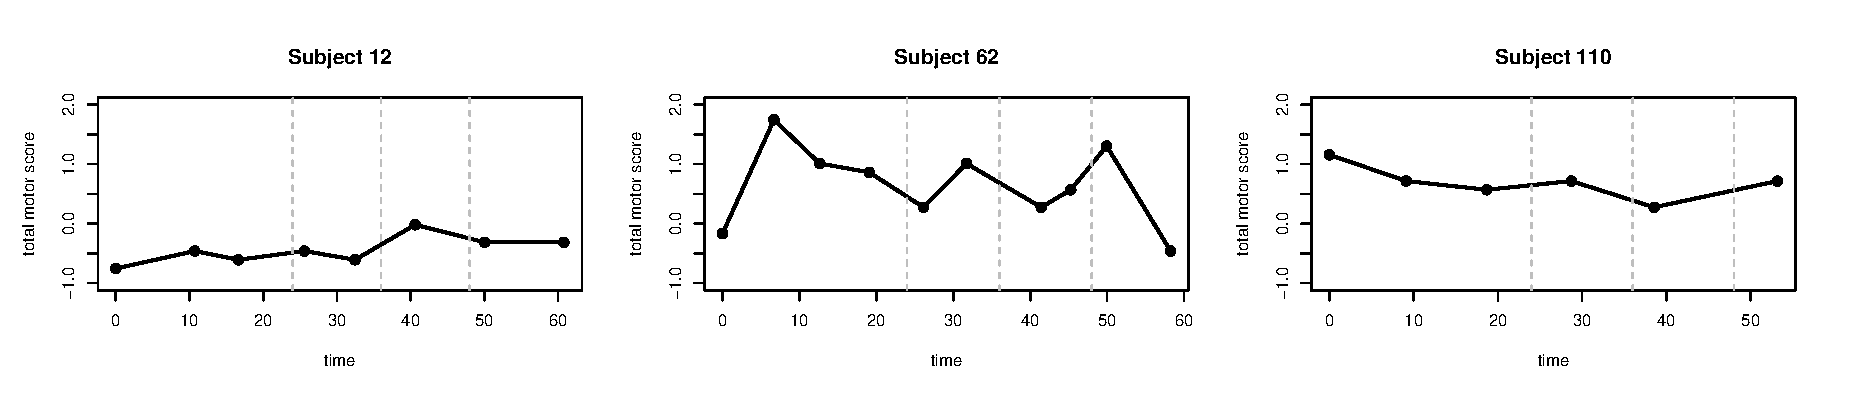
\includegraphics[width=\textwidth]{test_long_plot_12_62_110.eps}\label{plot:datafig11}
}

\subfloat[Predictions based on censoring time $t=$ 24 months]{
    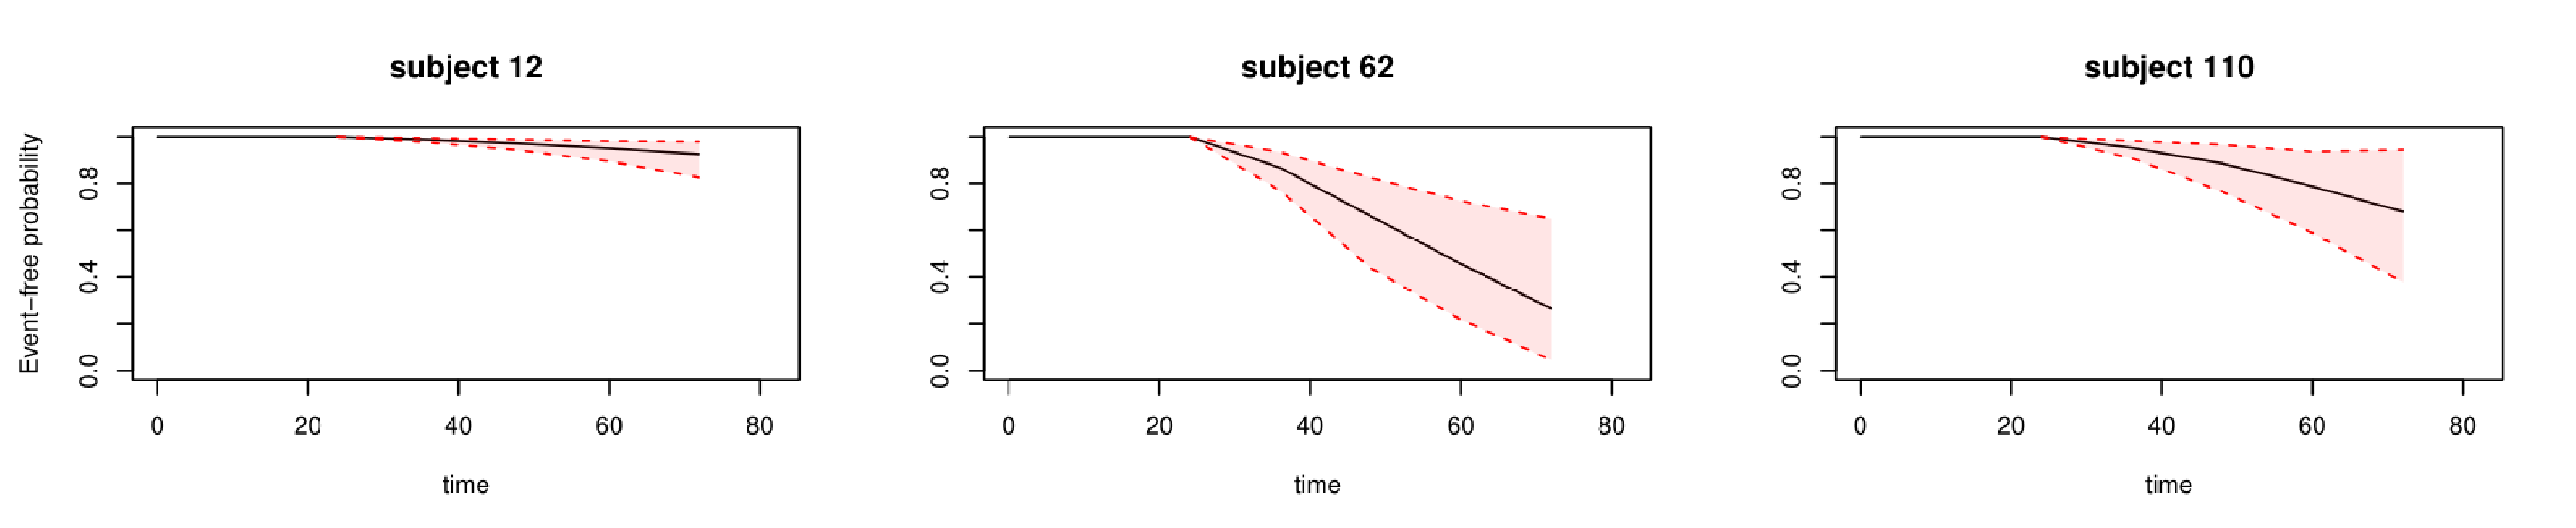
\includegraphics[width=\textwidth]{neurotot_qt50_pred_surv_t24_id_12_62_110.eps}\label{plot:datafig12}
}

\subfloat[Predictions based on censoring time $t=$ 36 months]{
    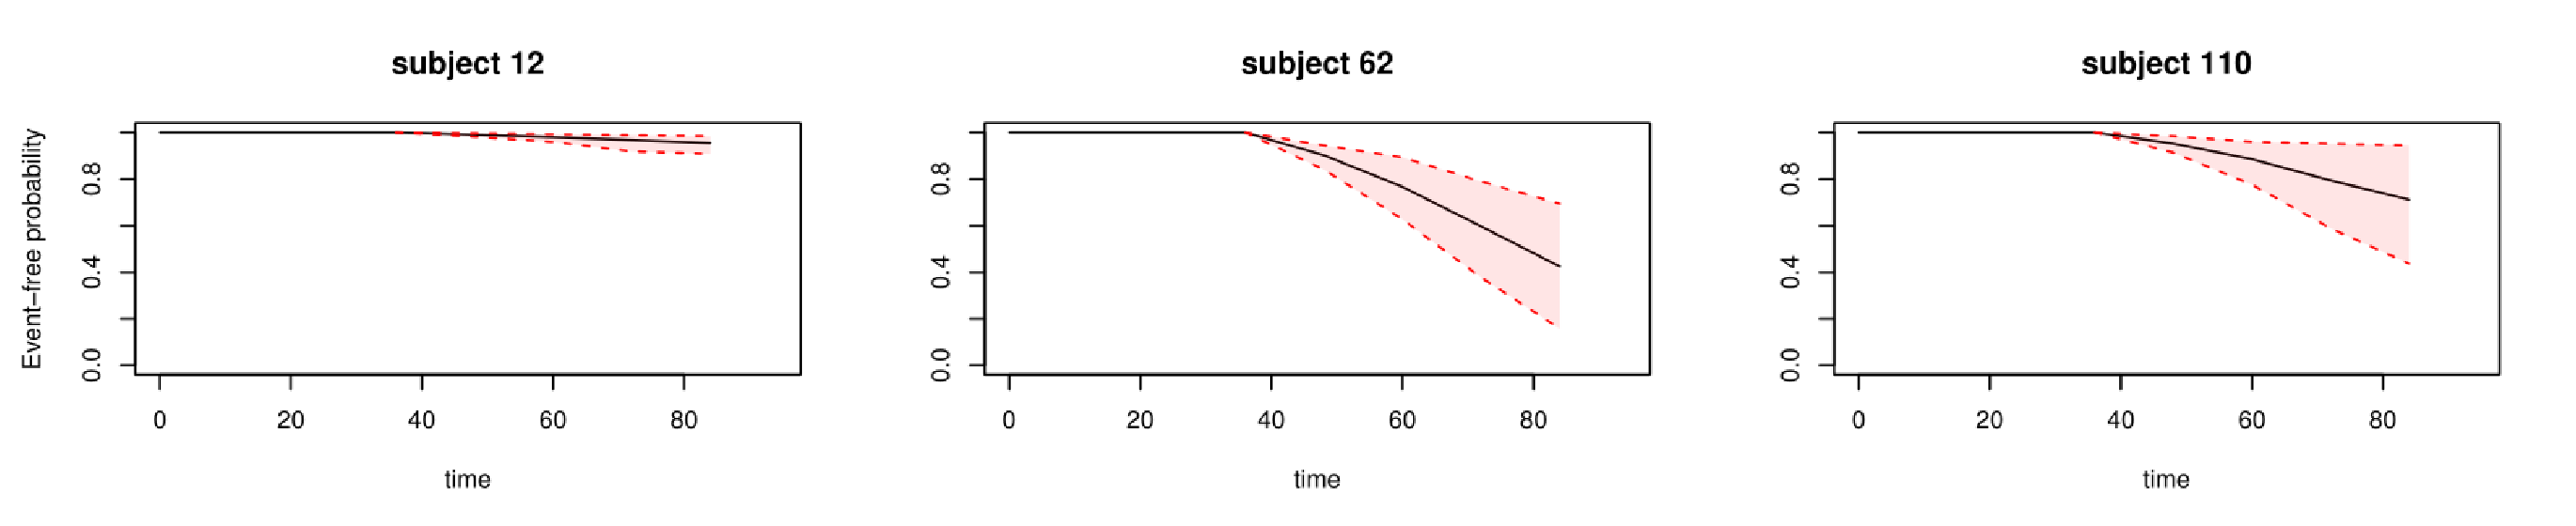
\includegraphics[width=\textwidth]{neurotot_qt50_pred_surv_t36_id_12_62_110.eps}\label{plot:datafig13}
}

\subfloat[Predictions based on censoring time $t=$ 48 months]{
    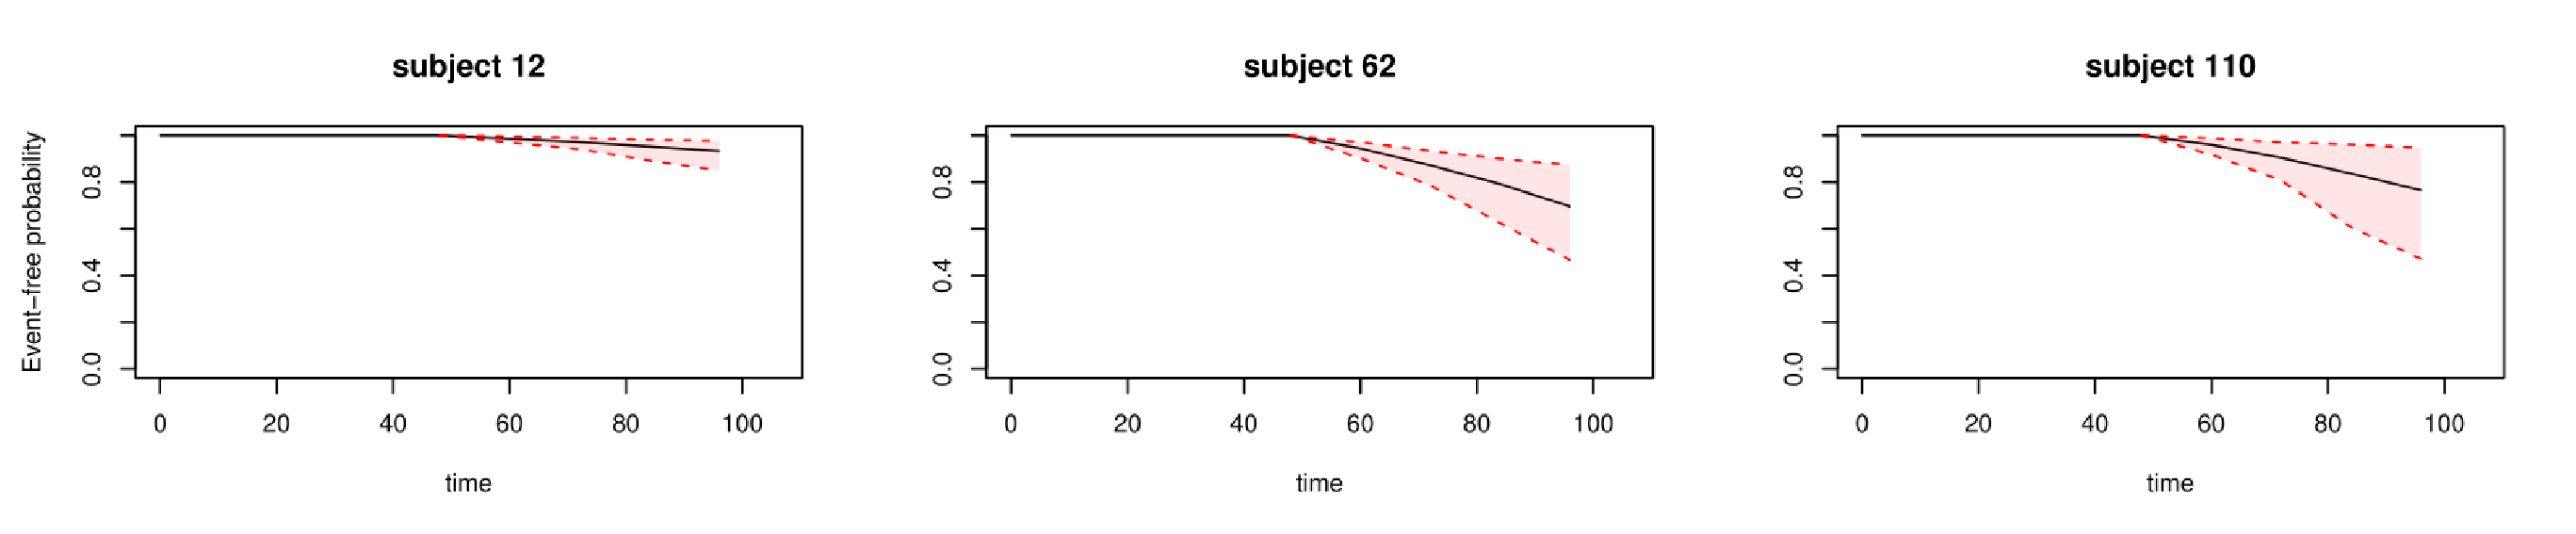
\includegraphics[width=\textwidth]{neurotot_qt50_pred_surv_t48_id_12_62_110.eps}\label{plot:datafig14}
}

  \caption{PREDICT-HD data analysis: Longitudinal trajectories and dynamic predictions of HD-free probabilities with 95\% pointwise credible interval from QRJM at $\tau=0.5$ for selected individuals.}
  \label{plot:datafig1}
\end{figure}

\subsection{Inference Results for PREDICT-HD data}\label{sec:data_results}
Finally, Table~\ref{p1realdata_inference} presents the inference result from the QRJMs with $\tau=0.25$, 0.50, and 0.75 and TMS as the longitudinal biomarker. In the longitudinal process, the coefficient for time quantifies the change rate of TMS at a fixed quantile. For example, Table~\ref{p1realdata_inference} suggests that the time effect is 0.019 (95\% CI: 0.015, 0.023) for TMS at $\tau=0.25$, indicating one month increase in time is associated with 0.019 unit increase of 25\% conditional quantile of TMS. The positive time coefficients for TMS at all quantiles indicate that TMS increases (deteriorates) over time, which is consistent with the loess curve in Figure~\ref{fig:data_neurotot} (upper panel). The magnitude of the time coefficients is similar at different quantiles of TMS, indicating comparable progression at those quantiles.

Table~\ref{p1realdata_inference} also suggests that higher baseline age is associated with higher (worse) TMS and one year increase in baseline age is associated with 0.004 (95\% CI: 0.001, 0.008) units increase in TMS at $\tau=0.5$. In the time to HD onset process, across all three quantiles, education has protective effect on HD onset, i.e., those with more education years tend to have a lower risk of HD onset. Outcome TMS is strongly predictive of HD onset at all quantiles. Specifically, an unit increase in TMS increases the risk of HD onset by 4.600 ($e^{1.526}$, 95\% CI 3.747-5.726) times at $\tau=0.25$, by 3.669 (95\% CI 3.152-4.302) times at $\tau=0.5$, and by 2.945 (95\% CI 2.633-2.294) times at $\tau=0.75$, respectively.


\begin{table}[ht]
\centering
\caption{PREDICT-HD data analysis: Parameter estimation and 95\% credible interval (in parenthesis) from QRJM at three different quantiles with TMS being the longitudinal biomarker.}
\label{p1realdata_inference}
\resizebox{\linewidth}{!}{
\begin{tabular}{lrrr}
  \hline
  & \multicolumn{1}{c}{$\tau=0.25$} & \multicolumn{1}{c}{$\tau=0.50$} & \multicolumn{1}{c}{$\tau=0.75$} \\
\hline
\multicolumn{4}{l}{For longitudinal TMS process}\\
Intercept & $-$0.760 ($-$0.903, $-$0.628)& $-$0.525 ($-$0.699, $-$0.359)& $-$0.249 ($-$0.469, $-$0.035)\\
Time (months) & 0.019 (0.015, 0.023)& 0.020 (0.016, 0.024)& 0.022 (0.018, 0.026)\\
Age & 0.004 (0.001, 0.008)& 0.005 (0.001, 0.010)& 0.006 (0.001, 0.012)\\ \\
\multicolumn{4}{l}{For time to HD onset process}\\
Education (years) & $-$0.083 ($-$0.115, $-$0.052)& $-$0.112 ($-$0.142, $-$0.082)& $-$0.128 ($-$0.157, $-$0.101)\\

Male & 0.317 ($-$0.037, 0.654)& 0.360 ($-$0.020, 0.708)& 0.317 ($-$0.010, 0.647)\\
Association & 1.526 (1.321, 1.745)& 1.300 (1.148, 1.459)& 1.080 (0.968, 1.192)\\
  \hline
\end{tabular}
}
\end{table}


\section{Discussion}\label{sec:discussion}
In our application of the linear-mixed joint model (LMJM, a linear mixed sub-model for the longitudinal process and a Cox sub-model for the survival process) to Huntington's Disease, there are two limitations. First, the normality assumption of the random errors in the linear mixed model (LMM) was not realistic, and no obvious transformation of the longitudinal outcome to produce residual normality was applicable. This limitation is confirmed by our simulation studies where the LMJM tends to provide biased estimates to model parameters when the longitudinal data are non-normal (skewed and /or heavy-tailed). Consequently, predictive accuracy of the LMJM is negatively impacted. Second, the LMJM only models the conditional mean of the outcome. However, in our (and other) clinical research application(s), it may be more clinically relevant to consider the tails of the outcome distribution, e.g., the upper tail of TMS is at higher risk of developing HD.

Our proposed quantile regression joint models (QRJM) uses a linear quantile mixed model (LQMM) for the longitudinal process, improves both inference and the ability to make accurate dynamic predictions. The quantile-based estimators are more robust against skewness in the data. Thus, our approach provides the flexibility to use median or quantile regression instead of mean regression when outliers and skewness are present in the longitudinal process. Moreover, the QRJM provides quantile-specific parameter estimates at a set of different quantiles and the researchers can choose the quantiles of interest and the corresponding inference results. The simulation studies and data application suggest that the QRJM not only inherits the good properties of an LMJM, but adds flexibility to the modeling procedure.

In this work, we develop a Bayesian algorithm to fit the proposed QRJM model and make dynamic predictions using the location-scale representation of the asymmetric Laplace distribution (ALD) for the longitudinal quantile regression. The Bayesian algorithm, which is straightforwardly implemented in \texttt{JAGS} software, uses a piecewise constant baseline hazard function in the survival sub-model. However, other functional forms can also be considered and the integration of the hazard function can be approximated using numerical integration such as Simpson's rule. In the real data application, we illustrate the flexibility of the QRJM and its advantages over the LMJM by jointly modeling the risk of developing HD and total motor score (TMS, a commonly used early predictor of HD). The QRJM is able to provide more insight into the disease progression and the association between the two disease processes in terms of various quantile-based estimations and dynamic predictions.

The novel application of our proposed QRJM in making personalized dynamic predictions of survival probability finds practical importance in many clinical applications. Event prediction using commonly collected biomarkers can provide clinicians with continuously updated ``disease progression'' information potentially allowing them to make appropriately timed intervention decisions for each individual. Subject-specific dynamic predictions models play an important role in the ongoing transformation of traditional medicine to personalized care. While in traditional medicine, treatment selection is guided by population-based experience, i.e., the average treatment effect in the entire population, such ``one-size-fits-all'' approaches are criticized for resulting in low efficacy and high adverse drug reactions in many clinical studies. Utilizing the dynamic predictions based on the proposed QRJM framework, we obtain subject-specific predictions of event risk that would actually allow physicians to tailor medical treatment based on a specific patient profile.

In summary, the QRJM is a good alternative to the LMJM when either the normality assumption of the errors term is concerned or the conditional quantiles are more relevant to the research questions. When the interest lies in the prediction of future survival probability, the ``best'' quantile may be chosen based on the predictive accuracy criteria. Other model selection methods or methods, e.g., Bayesian model averaging, to incorporate multiple regression results from different quantiles into a single prediction solution can be a potential direction for future work. However, in our opinion, the choice of specific quantile(s) should be more clinically oriented rather than be a statistical task.


\section*{Acknowledgements}
Sheng Luo's research was supported by the National Institute of Neurological Disorders and Stroke under Award Number R01NS091307. The authors acknowledge the Texas Advanced Computing Center (TACC) for providing high-performing computing resources. URL: \verb"http://www.tacc.utexas.edu".
\bibliographystyle{SageV}
\bibliography{paper1}


\end{document}
